\documentclass[12pt]{article}

\usepackage{fullpage}

\usepackage{mathspec}
\setmainfont[Mapping=tex-text]{Linux Libertine}
%\setmathfont(Digits,Greek,Latin){Garamond}

\usepackage[usenames,dvipsnames]{color}
\usepackage[colorlinks=true, urlcolor=NavyBlue]{hyperref}
\usepackage{graphicx}

\title{Mapping basics in R, a brief tutorial}
\author{Hilary Prichard (the good parts) and Aaron Ecay (the rest)}
\date{\today}

\begin{document}
\maketitle

\section{Purpose}

This tutorial will guide you through the basics of mapping in R, from creating a geocoded data frame to mapping values as points. Links describing more advanced mapping techniques for you to explore are also included at the end of this tutorial. There are two accompanying files: \texttt{telsur-example.csv} is a file with sample data taken from the Atlas of North American English which we will be using to produce an ANAE-style map; \texttt{telsur-example.R} is a file with the R code for creating the map.

\section{Data structure}

In order to create a map, you first need to collect two different kinds of data: linguistic data, and geographic data.

``Linguistic data" is the dialect data you will find in the dialect atlas you choose, and it can take whatever form you like -- phonetic transcriptions, coded variables, percentages, etc. ``Geographic data" is the latitude and longitude data that allows R to put your dialect data on a map. In the unlikely event that your dialect data is already coded with the latitude and longitude of each location, you're good to go! Most of you, however, will need to \emph{geocode} your data, using whatever location identifiers you have on hand, like city, state, county, or zip code.

The end goal is a spreadsheet with (minimally) columns for latitude, longitude, and linguistic variable. For example, the data we'll be working with in this tutorial looks like this:

\begin{figure}[h]
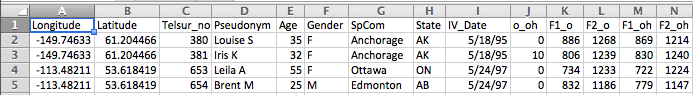
\includegraphics[width=\linewidth]{data.png}
\end{figure}

\noindent We have columns for latitude and longitude, and five columns for linguistic information. Column ``o\_oh" is a perception test score, while ``F1\_o" through ``F2\_oh" contain vowel formant measurements.

If you have more data than is feasible to geocode by hand, one option is to use \url{http://www.gpsvisualizer.com/convert_input}.

If you already have zip codes for your data, and you're comfortable working in R, another option is to use the \texttt{zipcode} package. This package contains a function which checks the format of your zip codes, and a data frame of latitudes and longitudes for each zip code. You can use \texttt{merge} to get latitude and longitude for your zip codes.

Once your data is collected and geocoded, save it as a .csv (comma-separated values) file so that you can easily work with it in R.

\section{Getting started with R}
If you've never used R before, I strongly recommend having a look at Joe Fruehwald's study group materials, at \url{http://www.ling.upenn.edu/~joseff/rstudy/index.html}. While the example code provided here does not assume any prior experience with R, it would be helpful to have a basic understanding of how R works for following along and later adapting the code to your specific needs. Weeks 1 and 2 of Joe's tutorial should get you up to speed on the basics.

\section{The \texttt{ggplot2} package}

R comes with facilities for making graphs, including maps.  However,
experience shows that they are not always easy to use: the command for
creating one kind of graph may have little relation to the command for
another; parameters have somewhat cryptic names; etc.  Luckily, there is
another way: the \href{http://ggplot2.org/}{\texttt{ggplot2}}
package.\footnote{\texttt{ggplot} stands for “Grammar of Graphics” plot;
    a notion which should appeal to us linguists.}  The
\href{http://www.cookbook-r.com/Graphs/}{Cookbook for R} website’s
section on graphs has many applied examples of using ggplot to make
several kinds of graphs (but not maps, sadly!)

The example code attached shows you how to create maps in R using \texttt{ggplot2} and the \href{http://cran.r-project.org/web/packages/maps/maps.pdf}{\texttt{maps} package}. We will be using the ``state" map in this tutorial; this gives us a pre-defined map of the U.S. with state boundaries. Other pre-defined maps are available via this package (see documentation), but should the area you're working on not be included in this way, you can always use the ``world" map and set your x and y axis limits to only plot the part of the world you're interested in.

An alternative to \texttt{maps} is \texttt{mapdata}, which contains higher-resolution world maps but fewer pre-defined country maps. The documentation for \texttt{mapdata} is here: \url{http://cran.r-project.org/web/packages/mapdata/mapdata.pdf}.

\section{On to the code!}
Now that we've covered the preliminaries, let's look at an example of how to build a basic map in R. You will need:
\begin{enumerate}
\item The current version of R (\url{http://lib.stat.cmu.edu/R/CRAN/}) or RStudio (a much nicer user interface for R: \url{http://www.rstudio.com/})
\item The \texttt{maps}, \texttt{ggplot2}, and \texttt{ggmap}
  packages. In R, do: \texttt{install.packages(c("maps", "ggplot2", "ggmap"))}
\end{enumerate}

Once you have those, open up \texttt{telsur-example.R} in R. For anyone unfamiliar with what R code looks like, all the grey lines with a pound symbol (\#) at the beginning are my commentary and instructions. All other lines are for you to copy/paste into your R prompt. On a Mac, you can also highlight a line of code and hit Command + Enter to execute it.

Read through \texttt{telsur-example.R}, executing the lines of code as instructed. I've included lots of comments explaining what each piece does, but if you want to read more about the functions used in the code, you can access the R help documents by typing a question mark in front of a function name. For example, type in \texttt{?fortify} for more information on ggplot’s \texttt{fortify} function.

When you get to the end, if everything has gone well, you should have a pdf that looks like this:
\begin{figure}[h]
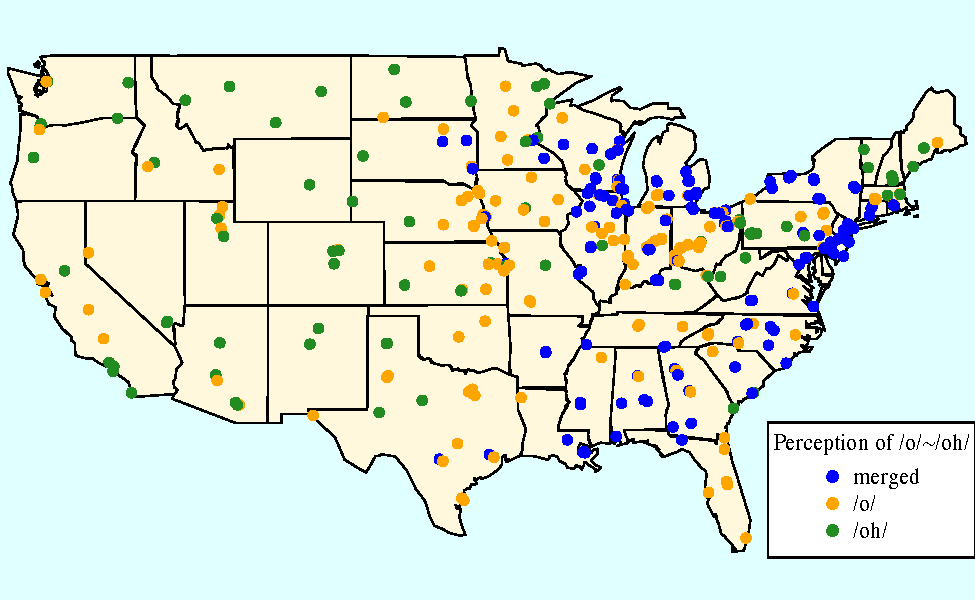
\includegraphics[width=\linewidth]{telsur-example.pdf}
\end{figure}

Hooray!

\clearpage
\section{Further resources}
\subsection{You have questions, the internet has answers}
If you ever have a question about how to do something in R that isn't covered in the help documents, chances are someone else has had the same question, and posted it on \url{http://stackoverflow.com/}. Checking Stack Overflow and googling error messages will most often get you the answer you need.

I've already mentioned Joe Fruehwald's R Study Group materials, but I'll mention them again. \href{http://jofrhwld.github.io/rstudy/summer2010_ggplot2_intro.html}{His ggplot intro} has a thorough introduction to ggplot with many examples..

\subsection{More advanced mapping to explore}
\begin{enumerate}
\item Topography: Terrain maps can be created with \texttt{RgoogleMaps}:\\ \url{http://www.molecularecologist.com/2012/09/making-maps-with-r/}
\item Rivers: or just add rivers to a map using the "rivers" map in \texttt{mapdata}.
\item ggplot: The \texttt{ggplot2} package offers an alternative to mapping in base graphics, with all the features we love about regular ggplotting:\\
\url{http://docs.ggplot2.org/current/geom_map.html}\\
Or explore \texttt{ggmap} for integration with Google Maps and OpenStreetMap:\\
\url{http://cran.r-project.org/web/packages/ggmap/ggmap.pdf}
\item Choropleth maps are another attractive option, when it would be more appropriate to color-code entire counties or states rather than plotting individual points. This blog post has a variety of solutions to the same mapping problem:\\
\url{http://blog.revolutionanalytics.com/2009/11/choropleth-challenge-result.html}
\item Animated gifs! Not just for buzzfeed anymore. Aaron Ecay has been exploring the use of animated maps to display diachronic change in syntactic variables. You should talk to him if this seems like something you'd be interested in doing.
\end{enumerate}

\end{document}
